\section{Starting and stopping Pbinds independently}

This is a very common question that comes up about \texttt{Pbind}s, especially the ones that run forever with \texttt{inf}: how can I stop and start individual \texttt{Pbind}s at will? The answer will involve using variables, and we'll see a complete example soon; but before going there, we need to understand a little more of what happens when you play a \texttt{Pbind}.

\subsection{Pbind as a musical score}

You can think of \texttt{Pbind} as a kind of musical score: it is a recipe for making sounds, a set of instructions to realize a musical passage. In order for the score to become music, you need to give it to a player: someone who will read the score and make sounds based on those instructions. Let's conceptually separate these two moments: the definition of the score, and the performance of it. 

 
\begin{lstlisting}[style=SuperCollider-IDE, basicstyle=\scttfamily\footnotesize]
// Define the score
(
p = Pbind(
	\midinote, Pseq([57, 62, 64, 65, 67, 69], inf),
	\dur, 1/7
); // no .play here!
)

// Ask for the score to be played
p.play;
\end{lstlisting}
 

The variable \texttt{p} in the example above simply holds the score---notice that the \texttt{Pbind} does not have a \texttt{.play} message right after its closing parenthesis. No sound is made at that point. The second moment is when you ask SuperCollider to play from that score: \texttt{p.play}.

A common mistake at this point is to try \texttt{p.stop}, hoping that it will stop the player. Try it and verify for yourself that it doesn't work this way. You will understand why in the next couple of paragraphs.

\subsection{EventStreamPlayer}

Clean the Post window with [ctrl+shift+P] (not really needed, but why not?) and evaluate \texttt{p.play} again. Look at the Post window and you will see that the result is something called an \texttt{EventStreamPlayer}. Every time you call \texttt{.play} on a \texttt{Pbind}, SuperCollider creates a player to realize that action: that's what \texttt{EventStreamPlayer} is. It's like having a pianist materialize in front of you every time you say ``I want this score to be played right now.'' Nice, huh?

Well, yes, except that after this anonymous virtual player shows up and starts the job, you have no way to talk to it---it has no name. In slightly more technical terms, you have created an object, but you have no way to refer to that object later. Maybe at this point you can see why doing \texttt{p.stop} won't work: it's like you are trying to talk to the score instead of talking to the player. The score (the \texttt{Pbind} stored in the variable \texttt{p}) knows nothing about starting or stopping: it is just a recipe. The \emph{player} is the one who knows about starting, stopping, ``would you please take from the beginning'', etc. In other words, you have to talk to the \texttt{EventStreamPlayer}. All you need to do is to give it a name, in other words, store it into a variable:

 
\begin{lstlisting}[style=SuperCollider-IDE, basicstyle=\scttfamily\footnotesize]
// Try these lines one by one:
~myPlayer = p.play;
~myPlayer.stop;
~myPlayer.resume;
~myPlayer.stop.reset;
~myPlayer.start;
~myPlayer.stop;
\end{lstlisting}
 

In summary: calling \texttt{.play} on a \texttt{Pbind} generates an \texttt{EventStreamPlayer}; and storing your \texttt{EventStreamPlayer}s into variables allows you to access them later to start and stop patterns individually (no need to use [ctrl+.], which kills everything at once).

\subsection{Example}

Here's a more complex example to wrap up this section. The top melody is borrowed from Tchaikovsky's Album for the Youth, and a lower melody is added in counterpoint. Figure \ref{fig:counterpoint} shows the passage in musical notation.
 
%\lstinputlisting[style=SuperCollider-IDE, basicstyle=\scttfamily\footnotesize]{code-pbind-start-stop.scd}

\begin{lstlisting}[style=SuperCollider-IDE, basicstyle=\scttfamily\footnotesize]
// Define the score
(
var myDurs = Pseq([Pn(1, 5), 3, Pn(1, 5), 3, Pn(1, 6), 1/2, 1/2, 1, 1, 3, 1, 3], inf) * 0.4;
~upperMelody = Pbind(
	\midinote, Pseq([69, 74, 76, 77, 79, 81, Pseq([81, 79, 81, 82, 79, 81], 2), 82, 81, 79, 77, 76, 74, 74], inf),
	\dur, myDurs
);
~lowerMelody = Pbind(
	\midinote, Pseq([57, 62, 61, 60, 59, 58, 57, 55, 53, 52, 50, 49, 50, 52, 50, 55, 53, 52, 53, 55, 57, 58, 61, 62, 62], inf),
	\dur, myDurs
);
)
// Play the two together:
(
~player1 = ~upperMelody.play;
~player2 = ~lowerMelody.play;
)
// Stop them separately:
~player1.stop;
~player2.stop;
// Other available messages
~player1.resume;
~player1.reset;
~player1.play;
~player1.start; // same as .play
\end{lstlisting}

\begin{figure}[h]
\centerline{\framebox{
	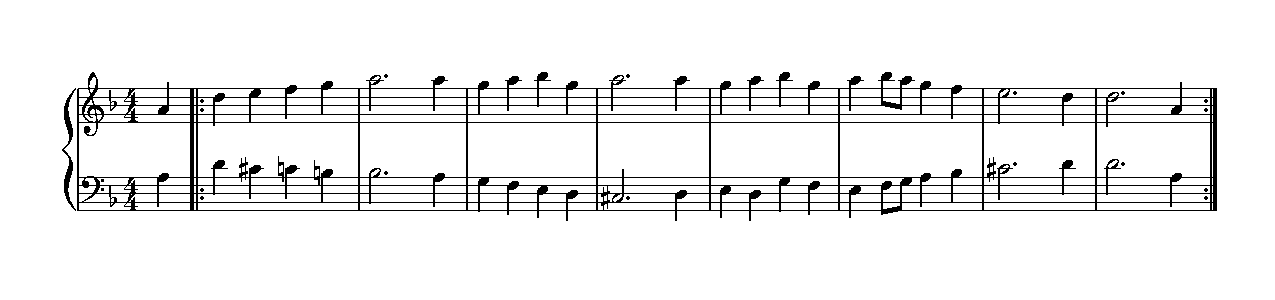
\includegraphics[scale=0.7]{code-pbind-start-stop-notation.pdf}}}
\caption{\texttt{Pbind} counterpoint with a Tchaikovsky melody}
\label{fig:counterpoint}
\end{figure}

First, notice the use of variables. One of them, \texttt{myDurs}, is a local variable. You can tell it's a local variable because it doesn't start with a tilde ($\sim$) and it's declared at the top with the reserved keyword \texttt{\textbf{var}}. This variable holds an entire \texttt{Pseq} that will be used as \texttt{\textbackslash dur} in both of the \texttt{Pbind}s. \texttt{myDurs} is really only needed at the moment of defining the score, so it makes sense to use a local variable for that (though an environment variable would work just fine too). The other variables you see in the example are environment variables---once declared, they are valid anywhere in your SuperCollider patches.

Second, notice the separation between score and players, as discussed earlier. When the \texttt{Pbind}s are defined, they are not played right away---there is no \texttt{.play} immediately after their closing parenthesis. After you evaluate the first code block, all you have is two \texttt{Pbind} definitions stored into the variables \texttt{$\sim$upperMelody} and \texttt{$\sim$lowerMelody}. They are not making sound yet---they are just the scores. The line \texttt{$\sim$player1 = $\sim$upperMelody.play} creates an \texttt{EventStreamPlayer} to do the job of playing the upper melody, and that player is given the name $\sim$player1. Same idea for $\sim$player2. Thanks to this, we can talk to each player and request it to stop, start, resume, etc.

At the risk of being tedious, let's reiterate this one last time:
\begin{itemize}
\item A \texttt{Pbind} is just a recipe for making sounds, like a musical score;
\item When you call the message \texttt{play} on a \texttt{Pbind}, an \texttt{EventStreamPlayer} object is created;
\item If you store this \texttt{EventStreamPlayer} into a variable, you can access it later to use commands like \texttt{stop} and \texttt{resume}.
\end{itemize} 